
% Rules for the HuroCup United Competition
% Jacky Baltes <jacky@cs.umanitoba.ca> 

\documentclass[12pt]{hurocup}

\newcommand{\thisyear}{2010}

\newcommand{\HuroCup}{\textsc{HuroCup}}


\begin{document}

\title{\HuroCup: Soccer\\
Laws of the Game \thisyear}

\author{Jacky Baltes\\
Autonomous Agents Laboratory\\
University of Manitoba\\
Winnipeg, Manitoba\\
Canada, R3T 2N2\\
Email: jacky@cs.umanitoba.ca\\
WWW: http://www.cs.umanitoba.ca/\~{ }jacky\\[5mm]
Kuo-Yang Tu\\
National Kaohsiung First University of Science and Technology\\
Kaohsiung City, R. O. C.\\
Email: tuky@ccms.nkfust.edu.tw\\[5mm]
Sock Lip Lim\\
Nanyang Polytechnic\\
Singapore, Singapore\\
Email: lim\_sock\_lip@nyp.gov.sg 
}

\maketitle
\begin{abstract}
The following rules and regulations govern the united event in
\HuroCup, a robotic game and robotics benchmark problem for humanoid
robots. The emphasis in the united competition is on collaboration
with robots from other teams. A common extensible communication
framework based on 802.11 b/g/n allows teams to communicate their
state, perceptions, and intentions.
%
\end{abstract}

\section*{Latest Version of the Rules for \HuroCup}
\label{sec:updates}

The latest official version of the rules of the game for \HuroCup\ is
always available from the \HuroCup\ Facebook page
(http://www.facebook.com/groups/hurocup/).

\section*{Changes to the Rules of \HuroCup\ United for \thisyear}

The \HuroCup\ United competition will be held for the first time in
2012.

\newpage

\section*{United Soccer}
\label{sec:soccer}

The following rules govern the game of \HuroCup\ United
competition. The rules are based on the \HuroCup\ rules as well as the
FIFA rules.

In the United Soccer competition soccer teams will be formed by
randomly assigning players to teams with a maximum of five
robots. Therefore, robots must collaborate with unknown players from
other teams to play soccer well.

The goal of the United Soccer event is to develop the necessary
technology that will allow us to quickly increase the size of the
teams to 11 players each.

\section*{Laws of the Game}
\label{sec:laws}

The following laws are intended for humanoid robot soccer. As such,
they provide a background and further information for the laws of the
individual events.

\law[US]{The Field of Play}
\label{law:field-of-play}

\begin{lawlist}[US]
  
\item The playing surface is a hardwood surface or a carpet. The floor
  under the surface is level, flat and hard.

\item The colour of the playing field is green.
  
\item Dimensions: The length of the field must be rectangular. The
  length of the field (touch line) must be greater than the width of
  the field (goal line). The length of the field must be greater than
  600cm and less than 700cm. The width of the field must be greater
  than 400cm and less than 500cm.
 
\item There is a 30cm wide boundary around the playing field. The
  boundary area is \emph{not} part of the playing field. Its purpose
  is to prevent damage to robots leaving the playing field.
 
\item The field of play is marked with lines. These lines belong to
  the area of which they are boundaries. The two longer boundary lines
  are called touch lines. The two shorter ones are called goal lines.

\item All lines are marked in white colour and are between 4.5 cm to
  5.5cm wide.

\item The field of play is divided into two halves by a half way
  line. 

\item The centre mark is indicated at the midpoint of the half way
  line. A circle with a diameter of 100cm is marked around it.
  
\item A figure of one possible legal playing field is shown in
  Fig.~\ref{fig:field-hurocup}.
  
  \begin{figure}
    \begin{center}
      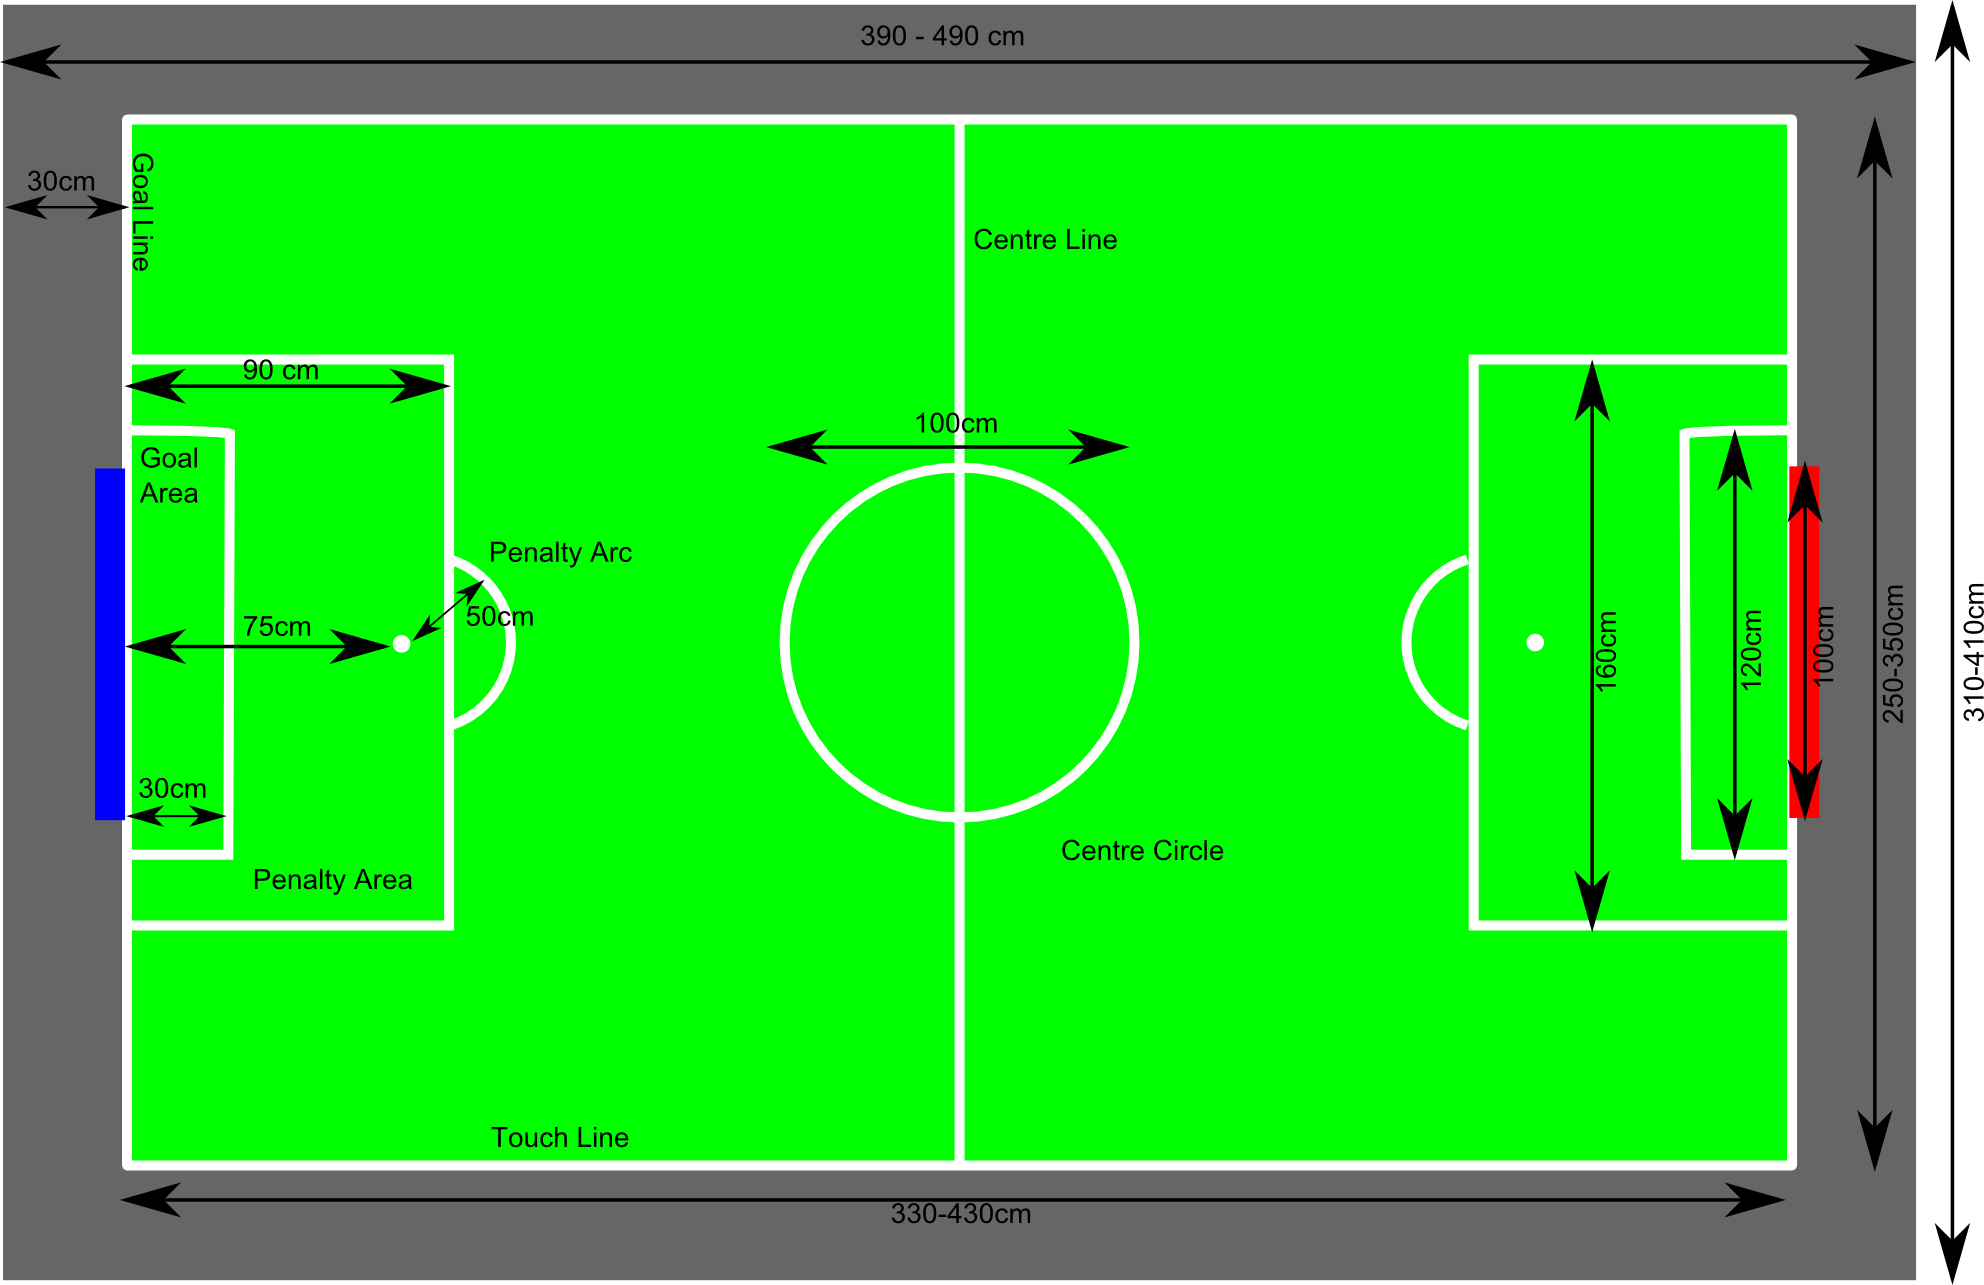
\includegraphics[width=0.8\textwidth]{Figures/hurocup-field}
      \caption{The field of play for \HuroCup\ United}
      \label{fig:field-hurocup}
    \end{center}
  \end{figure}
  
\item Goal Area: A goal area is defined at each end of the field as
  follows: Two lines are drawn at right angles to the goal line, 10cm
  from the inside of each goalpost. These lines extend into the field
  of play for a distance of 30cm and are joined by a line drawn
  parallel with the goal line. The area bounded by these lines and the
  goal line is the goal area.
  
\item Penalty Area: A penalty area is defined at each end of the field
  as follows: Two lines are drawn at right angles to the goal line,
  30cm from the inside of each goalpost. These lines extend into the
  field of play for a distance of 90cm and are joined by a line drawn
  parallel with the goal line. The area bounded by these lines and the
  goal line is the penalty area.
  
\item \label{penalty-mark} Penalty Mark: Within each penalty area, a
  penalty mark is made 75cm from the midpoint between the goalposts
  and equidistant to them.
  
\item \label{penalty-arc} Penalty Arc: The arc outside of the penalty
  area of the circle centred on the penalty mark and with a radius of
  50cm is drawn.

\item Goals must be placed on the centre of each goal line. They
  consist of two upright posts equidistant from the corner flag posts
  and joined at the top by a horizontal crossbar.
  
\item The distance between the posts is 200cm and the distance from
  the lower edge of the crossbar to the ground is 70cm. Both goalposts
  and the crossbar have the same width and depth which must be between
  5 to 10cm.
  
\item Nets may be attached to the goals and the ground behind the
  goal, provided that they are properly supported and do not interfere
  with the goalkeeper.
  
\item The goal posts and crossbar of the goal on one side of the
  playing field are coloured in red (the red goal).
  The goal posts and crossbar of the goal on the other side are
  coloured in blue (the blue goal).
  
\item Goals must be anchored securely to the ground. Portable goals
  may only be used if they satisfy this requirement.

\end{lawlist}

\begin{decisions}

\item In 2013, the size of teams will be increased to 7 players. In
  2014, we plan to play matches with 11 players per team.

\item The field of play shall be lighted by natural indoor
  lighting. The lighting should be as uniform as possible. The local
  organizing committee should attempt to provide information about the
  specific lighting conditions as early as possible to the
  competitors.
  
\item The specific colour and texture of the surface is not specified
  and may vary from competition to competition (just as real soccer
  fields vary). 

\item The surface underneath the carpet is level and
  hard. Examples of approved surfaces include: cement, linoleum,
  hardwood flooring, plywood, ping-pong tables and particle board;
  carpeted or cushioned surfaces are not allowed. Every effort shall
  be made to ensure that the surface is flat, however, it is up to
  individual teams to design their robots to cope with slight
  curvatures of the surface.

\end{decisions}

\law[US]{The Ball}
\label{law:ball}

\begin{lawlist}[US]
\item Robots in the \textit{small} category shall be using a yellow
 tennis ball.

\item Robots in the large category shall use an orange youth (Size 3)
soccer ball. 

\item If the ball becomes defective during the course of a match:
  \begin{itemize}
  \item the match is stopped,
  \item the match is restarted by placing the replacement ball at the place where the first ball became defective, 
  \item if the ball becomes defective whilst not in play at a
    kick-off, goal kick, corner kick, free kick, penalty kick or
    throw-in, then the match is restarted accordingly,
  \end{itemize}
\item the ball may not be changed during the match without the authority of the referee.

\end{lawlist}

\law[US]{Communication}
\label{law:communication}

\begin{lawlist}[US]

\item A wireless access point using the 802.11 g WIFI standard will be
  made available by the organizers.

\item The organizers will add a referee box that sends UDP broadcast
  messages to indicate the state of the game to all robots.

\item Only the robots themselves and the computing infrastructure by
  the organizing committee (referee box) are allowed to use the WIFI
  access point.

\item The robots are allowed to communicate via the following mediums
  only:
  \begin{enumerate}
  \item The WIFI access point provided by the organizers. All
    communication between the robots and the organizers should use
    UDP only.
  \item Robots may communicate via all other forms of human
    communication which includes gestures, speech, or sound. Speech
    and sound communication must be limited in time and volume.
  \end{enumerate}

\item \label{comm-limits} All robots must not use more than 10 KBytes
  of data per second. All robots must not send more than 30 messages
  per second.

\end{lawlist}

\law[US]{Number of Robots}

\begin{lawlist}[US]
\item A match is played with two teams, each consisting of not more
  than five players in the small category, and not more than three
  players for robots in the large category. One of the robots on each
  team is the goal keeper.

\item Only robots that are able to walk stably for a distance of at
  least one meter and that can get up from a fall within 30 seconds
  are deemed capable of play. The referee may ask the team to
  demonstrate the playing capability of the robot at any time during a
  stoppage in play. The referee will instruct the robot handlers to
  remove robots that are deemed incapable of play.

\item A maximum of two substitutes may be used in a game. A player
  that is substituting another player is only allowed to enter the
  field when the other player has left and when so instructed by the
  referee.

\end{lawlist}

\law[US]{Game Play}
\label{law:gameplay}

\begin{lawlist}[US]
\item At the beginning of the match, two teams will be formed by
  randomly selection of players.

\item At the start of the match, the referee toss a coin. The winner
  of the coin toss can decide on whether they would like to kick off
  in the first or in the second halt, or which side of the field the
  team would like to start on. The team that lost the coin toss can
  decide on the still open choice after the winner made its
  decision.
  
\item A match consists of two periods of play. Each period is ten
  minutes long.

\item A maximum five minute break (half-time) will start at the end of
  the first period.

\item After the end of the half time, the teams will switch their team jerseys
  and start side.

\item If a game ends in a draw, two additional periods of five minute
  duration with an additional five minute half-time will be played
  (Overtime). If at the end of the overtime the score is still tied,
  then the game will be decided by five alternating penalty kicks.

\item Each team can ask for a two minute time out. Each team has a
  maximum of two timeouts per game. At the beginning of the game or
  after a stoppage, a team which is unable to start must take a
  timeout, otherwise the referee will start the game without the team.

\end{lawlist}

\law[US]{Kick-Off}

\begin{lawlist}[US]

\item A kick-off will occur at the start of a period, after a goal has
  been scored, or after a time-out. If the kick-off occurs because a
  team has scored a goal, then the other team gets the kick-off. If a
  kick-off occurs because of a time-out, then the team that did not
  choose the time-out will have kick-off.

\item All robots that must be placed manually must be placed in such a
  way that at least one part of the robot's foot touches the goal
  area.

\item At the start of the kick-off, The referee will signal READY. The
  robots must move to their own half. If a robot can not reach its own
  half within 10 seconds, it must be placed manually by the robot
  handler.
  
\item All players of the opposing team must be outside of the centre
  circle. If a player of the opposing team violates this rule, then
  the robot must be placed manually. All human handlers must leave the
  field at the end of the READY phase.

\item After the READY phase, the referee will signal SET. Then the
  referee will place the ball on the centre spot. Robots must remain
  stationary during the SET phase. During the SET phase, the team
  taking the kick-off is allowed to place one robot inside of the
  centre circle to take the kick-off.

\item Approximately ten seconds after SET, the referee will signal
  PLAY by whistling and the assistant referee will send a PLAY message
  via UDP as well. The ball is in play when it is either touched by
  the player taking the kick-off or ten seconds have elapsed.

\item \label{ko-direct} A goal can not be scored directly from a
  kick-off. Either the ball must be moved by at least 20cm or be
  touched by another player before it is being kicked into the goal.
  If a team violates this rule, then a kick-off is awarded to the
  opposing team.

\end{lawlist}

\begin{decisions}
\item Note that given~\ref{ko-direct}, a goal will not be awarded if,
  for example, a robot kicks the ball directly from the kick-off
  position at the goal keeper and it then rolls into the goal. This is
  because the touch of the goal keeper occurred after the robot kicked
  the ball into the goal. However, if after the touch the goal keeper
  pushes it into its own goal, then it is a goal, since the touch
  occurred before it was kicked/pushed into the goal.
\end{decisions}

\law[US]{Dropped Ball}

\begin{lawlist}[US]
  \item A dropped ball is a way to restart a match from a neutral
    position should this be warranted.

  \item All robots must be placed outside of the centre circle when
    the referee signals READY. The referee will signal SET and place
    the ball at the centre point. Once the referee signals PLAY, the
    ball is in play and game continues.

  \item A goal can be scored directly from a dropped ball.

  \item If a robot enters the centre circle before the referee signals
    PLAY, a kick-off is awarded to the other team.
\end{lawlist}

\begin{decisions}
\item An example of a situation that warrants a Dropped Ball is, for
  example, if the ball is in such a position that none of the robots
  have sensed the ball or none of the robots have been able to move
  the ball.
\end{decisions}

\law[US]{Ball In and Out of Play}

\begin{lawlist}[US]
\item The ball is out of play when: (a) it has completely crossed the
  goal or touch line either on the ground or in the air, or (b) the
  game has been stopped by the referee.

\item At all other times, the ball is in play.
\end{lawlist}

\law[US]{Scoring a Goal}
\label{law:scoring}

\begin{lawlist}[US]
  
\item A goal is scored when the whole of the ball passes over the goal
  line, between the goal walls, below the crossbar, provided that the
  ball is in play and no infringement of the Laws of the Game has been
  committed previously by the team scoring the goal. 

\item A goal can not be scored by throwing the ball into the
  goal without touching another player first. This includes balls
  thrown by the opposing goal keeper or after a throw-in.
  
\item The team scoring the greater number of goals during a match is
  the winner. If both teams score an equal number of goals, or if no
  goals are scored, the match is a draw.
  
\item For matches ending in a draw, competition rules may state
  provisions involving extra time, or other procedures approved by the
  local organizing committee to determine the winner of a match.
\end{lawlist}

\law[US]{Untangling of Robots}

\begin{lawlist}[US]
\item \textbf{Untangling the Robots/No penalty}: If in the opinion of
  the referee there is immediate danger that two or more robots may be
  damaged through physical contact, s/he will instruct the robot
  handlers to pull the affected robots a distance of approximately
  50cm apart. The handlers must follow the instructions of the referee
  and must not alter the state of the robot unless instructed to do so
  by the referee.

\end{lawlist}

\begin{decisions}
\item When untangling the robots, the human handler is not allowed to
  stand up a fallen robot. Fallen robots must be laid down on the
  playing field. Furthermore, the handlers are not allowed to adjust
  the orientation of the robot.
\end{decisions}

\law[US]{Cautionable and Sending-Off Offences}
\label{law:cautionable}

\begin{lawlist}[US]

\item \textbf{Cautionable Offences/Yellow Card}: A team is cautioned
  and shown the yellow card if a robot on that team commits any of the
  following eight offences:
  \begin{enumerate}
    \item pushes an opponent
    \item holds an opponent
    \item strikes or attempts to strike an opponent
    \item charges an opponent
    \item damages or causes likely damage to another robot
    \item is guilty of unsporting behaviour
    \item modifies or damages the field, goal, or ball
    \item persistently infringes the Laws of the Game
  \end{enumerate}

\item \textbf{Sending-Off Offences/Red Card}: One robot is sent off
  and shown the red card if his team receives a second caution. The
  number of players on the team is reduced by one after every two
  yellow cards.

\end{lawlist}

\law[US]{Other Fouls and Misconduct}

\begin{lawlist}[US]

\item \textbf{Ball Manipulation/30 Sec. Removal}:It is an offence if the
  player, except the designated goal keeper within its goal area,
  manipulates the ball with any part of its hand, arm, or shoulder.

\item \textbf{Holding/30 Sec. Removal}: A single or a group of field
  players may not hold the ball for more than 1 second. The goal
  keeper in its own goal area may hold the ball for up to six
  seconds. It is considered holding the ball if no other robot has the
  ability to play the ball because either a single or multiple robots
  from the same team make it impossible to reach the ball for players
  from the other team.

\item \textbf{Physical Contact/30 Sec. Removal}: Physical contact
  between players from opposing teams must be avoided. In case of a
  collision, the faster moving robot will be penalized. No opposing
  player is allowed to touch the goal keeper in its own goal area.

\item \textbf{Incapacitated Player/30 Sec. Removal}: A robot that is
  unable to stand up within 30 seconds after a fall or a robot whose
  removal was requested by its robot handler must be removed. The
  referee will only grant removal of a malfunctioning robot if it does
  not lead to an advantage for its team.

\item \textbf{Charging/30 Sec. Removal}: A robot that is charging
  another robot and exerts significant force on it.

\item \textbf{Blocking The Goal/30 Sec. Removal}: A robot that blocks
  more than 50\% of the goal line for more than 15 seconds most of the
  time.

\item \textbf{Interference/30 Sec. Removal}: All robot handlers must
  remain outside of the playing field unless instructed by the
  referee. If the robot handler enters the playing field or interferes
  with the game in any way, the robot nearest to the handler will be
  removed.

\end{lawlist}

\begin{decisions}
\item The referee will not allow removal of a robot if it would result
  in an advantage for the team. For example, the referee will not
  allow removal of a robot lying in front of the goal and blocks a
  shot on goal by its team member.
\end{decisions}

\law[US]{Removal Penalty}
\label{law:removal penalty}

\begin{lawlist}[US]
\item A robot that commits any of the fouls mentioned above will be
  penalized by a removal penalty of 30 seconds.

\item When instructed by the referee, the robot handler must remove
  the robot as quickly as possible from the playing field without
  interfering with the remainder of the game.

\item After a removal penalty has expired, the robot may reenter the
  playing field. To reenter, the robot will be placed on one of the
  touch lines as closely as possible to the centre line without
  interfering with the rest of the game and the robot must face the
  centre circle. The referee will decide whether the robot must enter
  from the left or the right side.

\end{lawlist}

\begin{decisions}
\item The goal keeper must also enter from the centre line and walk
  back to the goal after it has received a removal penalty.
\end{decisions}

\law[US]{Penalty Kick}
\label{law:penalty-kick}

\begin{lawlist}[US]
  
\item A penalty kick is awarded if any of the seven offences for which
  a penalty kick may be awarded is committed by a robot inside his own
  penalty area, irrespective of the position of the ball, provided it
  is in play.
  
\item A goal may be scored directly from a penalty kick.
  
\item Additional time is allowed for a penalty kick to be taken at the
  end of each half or at the end of periods of extra time.
  
\item Procedure for a Penalty Kick: A penalty kick is taken by
  following this sequential procedure.
  \begin{enumerate}
    \item The ball is placed on the penalty mark
    \item  The defending goalkeeper is positioned so that some part of
      its construction touches the goalmouth line, facing the kicker,
      until the referee gives the start signal.
    \item The defending goal keeper must remain in a standard walking
      posture until the ball is kicked.
    \item The robot taking the penalty kick is: 
      \begin{itemize}
      \item properly identified,
      \item may be positioned by the team's designated robot handler.
      \end{itemize}
    \item The robots other than the kicker and the defending goalkeeper
      are located:
      \label{pk-other-players}
      \begin{itemize}
      \item inside the field of play,
      \item at least 15cm behind the penalty mark.
      \end{itemize}
    \item Where robots must be moved to comply with this law, the
      respective designated robot handlers may position them. The
      designated robot handler may always move the defending goalkeeper. 
    \item The Referee
      \begin{itemize}
      \item does not signal for a penalty kick to be taken until the
        robots have been placed in position in accordance with the Law,
      \item decides when a penalty kick has been completed.
      \end{itemize}
  \end{enumerate}   
  
\item The ball is in play when the referee signals the start of the
  penalty kick.
  
\item When a penalty kick is taken during the normal course of play,
  or time has been extended at half-time or full time to allow a
  penalty kick to be taken or retaken, a goal is awarded if the ball
  completely passes the goal line between the goalposts and under the
  crossbar.  even if the ball touches either or both of the goalposts
  and/or the crossbar, and/or the goalkeeper.

\item Infringements/Sanctions: \label{pk-infringements} If the referee
  gives the signal for a penalty kick to be taken and, before the ball
  is in play, one of the following situations occurs:

  The player taking the penalty kick infringes the Laws of the Game:
  \begin{itemize}
  \item the referee allows the kick to proceed,
  \item if the ball enters the goal, the kick is retaken,
  \item if the ball does not enter the goal, the kick is not retaken.
  \end{itemize}

  The goalkeeper infringes the Laws of the Game:
  \begin{itemize}
  \item the referee allows the kick to proceed,
  \item if the ball enters the goal, a goal is awarded,
  \item if the ball does not enter the goal, the kick is retaken.
  \end{itemize}

  A player of both the defending team and the attacking team
  infringe the Laws of the Game: the kick is retaken

  The ball is touched by an outside agent as it moves forward: the
  kick is retaken

  The ball rebounds into the field of play from the goalkeeper,
  the crossbar or the goalposts, and is then touched by an outside agent:
  \begin{itemize}
  \item the referee stops play,
  \item play is restarted with a dropped ball at the place where it
    touched the outside agent. 
  \end{itemize}
\end{lawlist}

\law[US]{Throw-In}
\label{us-throw-in}

A throw-in is a method of putting the ball back into play if it has
left the field by crossing either the touch lines or goal lines
(outside of the goal lines or above the cross bar) either on the
ground or in the air.

\begin{lawlist}[US]

\item A ball that has completely crossed the field line (either the
  touch line or the goal line outside of the goal posts or above the
  cross bar) results in a throw-in.

\item The game is not stopped for a throw-in.

\item The ball is as quickly as possible placed by the referee 50cm
  inside of the playing field at one of the touch lines. The position
  of the throw-in location along the touch lines is determined by the
  last robot to touch the ball before it went out of bounds.

\item \label{ti-min-dist} The throw-in location must not be closer
  than 1m to the goal line. If the throw-in location is closer than 1m
  to the goal line, the ball is placed at the nearest neutral location
  1m away from the goal line.

\item Within the restriction listed in ~\ref{ti-min-dist}, the
  location of the throw-in is determined using the following rules:
  \begin{enumerate}
    \item if the referee is unable to determine the last robot to
      touch the ball, then the ball is placed 50cm inside of the
      playing field at the nearest neutral position to where it has
      exited the playing field.
    \item if the referee can determine the last robot to touch the
      ball, then the ball is placed 50cm inside of the playing field
      at the location 1 m in the direction of the home goal of the
      offending robot.
    \item if a robot of the attacking team touches the ball last
      before it crosses the opponent's goal side outside of the goal
      posts or above the cross bar, then the throw in location is the
      nearest neutral location to the centre line.
  \end{enumerate}

\end{lawlist}

\law[US]{Scoring for Individual Players}

\begin{lawlist}[US]

\item A unique feature of the united soccer competition is the fact
  that in spite of soccer being a team sport, each player on the
  united team will receive an individual score.

\item After the match, the score for an individual player is
  calculated as follows. 

  \begin{center}
    \begin{tabular}{|l|r|}
      \hline
      Action & Points \\
      \hline
      Scoring a goal by a team mate   & +1\\
      The opposing team scored a goal & -1\\
      Scoring a goal                  & +5\\
      Making a save to prevent a goal & +3\\
      \hline
    \end{tabular}
  \end{center}

\end{lawlist}

\law[US]{Point Allocation}

\begin{lawlist}[US]
\item Any robot that has achieved less than one point is awarded $0$
  rank.

\item Among the robots that have at least one point, the robots are
  ranked (i.e., 1st place, 2nd place) based on the greater number of
  points.

\item In case of a tie, the number of goals scored by the robots are
  used as a tie breaker. If the robots have the same number of goals,
  the performance of the robot in the penalty kick competition will be
  used as a tie breaker.

\item The point allocation for robots is as follows:
  \begin{itemize}
  \item The first ranked robot is awarded $10$ points.
  \item The second ranked robot is awarded $8$ points.
  \item The third ranked robot is awarded $6$ points.
  \item The fourth, fifth, sixth, and seventh place robots are awarded
    $4$,$3$,$2$, and $1$ point respectively.  A summary of the point
    allocation for placings is shown in table~\ref{point-allocation}.

    \begin{table}
      \begin{center}
        \begin{tabular}{l|l}
          \hline
          Place & Points scored \\
          \hline
          1 (Winner) & 10 \\
          2          & 8 \\
          3          & 6 \\
          4          & 4 \\
          5          & 3 \\
          6          & 2 \\
          7          & 1 \\
          8, 9, ...  & 0 \\
          \hline
        \end{tabular}
      \end{center}
      \caption{Point allocation for placings}
      \label{point-allocation}
    \end{table}
  \end{itemize}

\item In case of a tie between $n$ robots with rank $k$, all robots
  will be awarded rank $k$ and receive the average of the scores for
  ranks $k$ to $k+n$.  For example, if the robots $A,B,C,D$ scored
  $10, 8, 8, 4$ points respectively, then robot $A$ will be declared
  the winner (1st place) and receive 10 points, both robots $B$ and
  $C$ will be declared 2nd place finishers and receive $(8+6)/2=7$,
  and robot $D$ will be declared the fourth place finisher and receive
  $4$ points.

\end{lawlist}

\section*{Appendix: Communication Protocol}

To improve the collaboration between the robots, all robots should
implement the following communication protocol. This allows robots
from different teams to exchange their state, perceptions, and
intentions.

The communication protocol is also used by the referee to transmit
data to the robots, such as the current state of the game.

All multi-byte data is send in most significant byte first (MSB) byte
order. 

The maximum message length allowed for a message is 65536 bytes.

All data is transmitted via UDP/IP broadcast messages. Since packet
delivery is not guaranteed using UDP/IP, certain message blocks may be
lost during communication. Robots must be able to function
autonomously even under conditions of severe package loss.

\subsection*{Message Format}

A message contains a header, the message length, the robot id, a
sequence number, the number of objects in the array, an array of
objects, and a check sum.

Each robot is assigned an ID. The robots defending the red goal will
receive IDs from 0 to 10. The robots defending the blue goal have IDs
16 to 26. A special ID (32) is assigned to the referee and messages
from the referee box.


\begin{center}
\begin{tabular}[t]{|l|l|p{0.3\linewidth}|}
  \hline
  Name & Type & Comment \\
  \hline
  Header          & UINT16 & 0xADDE\\
  Length          & UINT16 & Length of the message in bytes\\
  Robot ID        & UINT8 & Robot ID\\
  Sequence Number & UINT16 & Incremented for each message send by the
                             robot.\\
  Number of Objects & UINT8 & Number of objects in the message\\
  Objects & OBJECT[NUM\_OBJ] & The objects describing the state, perceptions,
                     and intentions of the robot\\
  Checksum & UINT8 & Sum of all bytes in the message excluding the
                     checksum itself\\
  \hline
\end{tabular}
\end{center}

\subsection*{Object Format}

The states, perceptions, and intentions of the robot are transmitted
using object messages.

All coordinates mentioned in a message are given in millimetres and
transmitted as signed 16 bit integers. The origin of the coordinate
system is the point where the goal line of the team's goal intersects
the touch line.

Positive direction of the X coordinate is along the touch
line. Positive direction of the Y coordinate is towards the home goal.

All orientation data is transmitted as a signed 16 bit integer in
radians multiplied by 10000 (RADIANS\_10000). For example, -18000
corresponds to an angle of $- 18023$ is equal to $1.8023$ radians or
approximately $-103$ degrees.

An angle of $0$ degrees is along the positive direction of the X axis
(touch line) and $90$ degree is along the goal line.

Each object has a confidence level associated with it. A robot can use
the confidence value to model how sure it is of this objects
information. A value of 255 indicates maximum confidence in the object
information.

\subsubsection*{State Object}

A state object describes the current state of the robot. This includes
an estimate of the robot's position, the ball positions, own team
robots, opponent team robots, and land marks. 

The state object can be used to transmit an estimated map of the
environment from the robot's point of view to the other robots on the
team.

The following shows the format of the state object.

\begin{center}
\begin{tabular}[t]{|l|l|p{0.3\linewidth}|}
  \hline
  Name & Type & Comment \\
  \hline
  Type          & UINT8 & 
  \begin{minipage}[t]{\linewidth}
    0 = UNDEFINED\\
    1 = Own position\\
    2 = Ball\\
    3 = Team Robot \\
    4 = Opponent Robot\\
    5 = Team Goal\\
    6 = Opponent Goal\\
  \end{minipage}\\
  Location X & INT16 & X location of the object in mm\\
  Location Y & INT16 & Y location of the object in mm\\
  Orientation & INT16 & Orientation of the robot in RADIANS\_10000\\
  Confidence & UINT8 & Confidence value\\
  \hline
\end{tabular}
\end{center}

\subsubsection*{Perception Object}

A robot can use a perception object to describe what it is currently
or has most recently sensed. If an object is not currently being
sensed then a state object must be used to transmit its information.

The following shows the format of the perception object.

\begin{center}
\begin{tabular}[t]{|l|l|p{0.3\linewidth}|}
  \hline
  Name & Type & Comment \\
  \hline
  Type          & UINT8 & 
  \begin{minipage}[t]{\linewidth}
    32 = UNDEFINED\\
    33 = Own Position\\
    34 = Ball\\
    35 = Team Robot \\
    36 = Opponent Robot\\
    37 = Team Goal\\
    38 = Opponent Goal\\
  \end{minipage}\\
  Location X & INT16 & X location of the object in mm\\
  Location Y & INT16 & Y location of the object in mm\\
  Orientation & INT16 & Orientation of the robot in RADIANS\_10000\\
  Confidence & UINT8 & Confidence value\\
  \hline
\end{tabular}
\end{center}

\subsubsection*{Intention Object}

The following shows the format of the intention object.

The offence value indicates the aggressiveness of the intention. A
maximum value of 255 would indicate a shot on goal, whereas a value of
0 would indicate a very defencive move such as trying to block a shot
on goal. A value of 128 indicates a neutral intention such as
receiving a pass.

\begin{center}
\begin{tabular}[t]{|l|l|p{0.3\linewidth}|}
  \hline
  Name & Type & Comment \\
  \hline
  Type          & UINT8 & 
  \begin{minipage}[t]{\linewidth}
    64 = UNDEFINED\\
    65 = Target location of movement\\
    66 = Play goal keeper\\
  \end{minipage}\\
  Location X & UINT16 & X location of the object in mm\\
  Location Y & UINT16 & Y location of the object in mm\\
  Orientation & INT16 & Orientation in RADIANS\_10000\\
  Offence & UINT8 & Aggressiveness of the intention\\
  \hline
\end{tabular}
\end{center}

\subsubsection*{Referee Objects}

A controller connected to the same wireless network will transmit
messages from the referee to the players.

This message includes a bitmask identifying which robots on each team
are currently in play or have been penalized with a 30 second removal
penalty. Any robot whose id bit is not set must remain motionless.

During \verb+Game Set+, all robots should remain motionless.

\begin{center}
\begin{tabular}[t]{|l|l|p{0.3\linewidth}|}
  \hline
  Name & Type & Comment \\
  \hline
  Type          & UINT8 & 
  \begin{minipage}[t]{\linewidth}
    96 = UNDEFINED\\
    97 = Game State\\
  \end{minipage}
  \\
  Team Red & UINT16 & Bitmask of players from the Red team that are
  allowed to play\\
  Team Blue & UINT16 & Bitmask of players from the Blue team that
  are allowed to play\\
  Time & INT16 & Remaining seconds in the period to play\\
  State & UINT8 & 
  \begin{minipage}[t]{\linewidth}
    0 = Game Stopped\\
    1 = Kick Off Red\\
    2 = Kick Off Blue\\
    3 = Game Set\\
    4 = Game Play\\
  \end{minipage}\\
  \hline
\end{tabular}
\end{center}

\subsubsection*{Extension Objects}

A team may use extension objects to transmit additional information as
long as it does not violate the bandwidth and transfer rate limits
described in section~\ref{comm-limits}.

To transfer larger proprietary data, multiple extension objects can be
transmitted in a message.

\begin{center}
\begin{tabular}[t]{|l|l|p{0.3\linewidth}|}
  \hline
  Name & Type & Comment \\
  \hline
  Type          & UINT8 & 
  \begin{minipage}[t]{\linewidth}
    96 = UNDEFINED\\
    97 = Game State\\
  \end{minipage}\\
  Proprietary1 & UINT16 & Extension data\\
  Proprietary2 & UINT16 & Extension data\\
  Proprietary3 & INT16 & Extension data\\
  Proprietary4 & UINT8 & Extension data\\
  \hline
\end{tabular}
\end{center}

\end{document}


% *** Local Variables: ***
% *** mode: LaTeX ***
% *** mode: outline-minor ***
% *** mode: auto-fill ***
% *** outline-regexp: "% !\\|\\\\\\(sub\\)*section" ***
% *** TeX-command-default: "LaTeX PDF" ***
% *** End: ***
